\documentclass[10pt, a4paper]{article}

\usepackage{graphicx}
\usepackage{listings}
\usepackage{color}
\usepackage{amsmath}
\usepackage{geometry}
\usepackage{setspace}
\usepackage{biblatex}
\usepackage{float}
\usepackage[hidelinks]{hyperref}
\usepackage{subcaption}
\usepackage[export]{adjustbox}
 
% Page master configuration
\lstset { basicstyle=\ttfamily, breaklines = true, tabsize=2 }
\geometry { a4paper, total={170mm,257mm}, left=20mm, top=20mm, right=20mm, bottom=20mm }
\graphicspath{{Images/}}
\addbibresource{biblography.bib}
\setlength{\parskip}{0.5em}
\setlength{\parindent}{0cm}
\setlength{\belowcaptionskip}{-10pt}

\definecolor{dkgreen}{rgb}{0,0.6,0}
\definecolor{gray}{rgb}{0.5,0.5,0.5}
\definecolor{mauve}{rgb}{0.58,0,0.82}

\lstset{frame=tb,
  language=Java,
  aboveskip=3mm,
  belowskip=3mm,
  showstringspaces=false,
  columns=flexible,
  basicstyle={\footnotesize\ttfamily},
  numbers=none,
  numberstyle=\tiny\color{gray},
  keywordstyle=\color{blue},
  commentstyle=\color{dkgreen},
  stringstyle=\color{mauve},
  breaklines=true,
  breakatwhitespace=true,
  tabsize=3
}

%%%%%%%%%%%%%%%%%%%%%%%%%%%%%%%%%%%%%%%%%%%%%%%%%%%%%%%%%%%%%%%%%%%%%%%%%%%%%%%%%%%%%%%%%%%%%%%%%%%%%%%%%%
\begin{document}

\begin{titlepage}
	\newcommand{\HRule}{\rule{\linewidth}{0.5mm}}
    
\includegraphics[scale=0.1]{./Images/Imperial_Logo.jpg} 
    \\
    \center 
	\textsc{\large Department of Electrical and Electronic Engineering }\\[0.5cm] 
	\textsc{\normalsize ELEC60030: Robotic Manipulation}\\[0.5cm] 
    
	\HRule \\[0.4cm]
	Team Machina: OpenMANIPULATOR-X Coursework Report
    \HRule \\[1.5cm]
     
    \begin{center}
		\underline{Authors}\\[0.5cm] 
        Khayle Torres \\ CID: 01753211 \\ kt1719@ic.ac.uk \\ [0.5cm]

        Xin Wang \\ CID: 01735253 \\ xw2519@ic.ac.uk \\ [0.5cm]
        
        Yuna Valade \\ CID: 01765409 \\ yv19@ic.ac.uk \\ [0.5cm]

	\end{center} \large

    \vfill 
    \makeatletter
    \@date 
    \makeatother
\end{titlepage}

%%%%%%%%%%%%%%%%%%%%%%%%%%%%%%%%%%%%%%%%%%%%%%%%%%%%%%%%%%%%%%%%%%%%%%%%%%%%%%%%%%%%%%%%%%%%%%%%%%%%%%%%%%
\renewcommand{\baselinestretch}{0.75}\normalsize
\tableofcontents
\renewcommand{\baselinestretch}{1.0}\normalsize

\pagebreak
%%%%%%%%%%%%%%%%%%%%%%%%%%%%%%%%%%%%%%%%%%%%%%%%%%%%%%%%%%%%%%%%%%%%%%%%%%%%%%%%%%%%%%%%%%%%%%%%%%%%%%%%%%

%%%%%%%%%%%%%%%%%%%%%%%%%%%%%%%%%%%%%%%%%%%%%%%%%%%%%%%%%%%%%%%%%%%%%%%%%%%%%%%%%%%%%%%%%%%%%%%%%%%%%%%%%%
\section{Task 1 - Modelling}

\subsection{Assigning Coordinate Frames}

The OpenMANIPULATOR-X robotic arm has 4-DOF and a 1-DOF gripper. The choice of
assigned coordinate frames to represent this robotic arm is important to how the
user would interact with the robotic arm. To assign the coordinate frames, there are several
important aspects the team took into consideration:
\begin{itemize}
    \item The team used
    CAD\footnote{\url{https://emanual.robotis.com/docs/en/platform/openmanipulator_x/specification}} 
    and
    Matlab\footnote{\url{https://uk.mathworks.com/matlabcentral/fileexchange/65316-designing-robot-manipulator-algorithms}}
    models of the robotic arm in order to obtain precise measurements
    and insight to how the robotic joints interacts.

    \item Where the robotic arm has a joint, the team assigned a coordinate
    frame to it as shown in the images below 
    \begin{figure}[h!]
      \centering
      \begin{subfigure}{.5\textwidth}
        \centering
        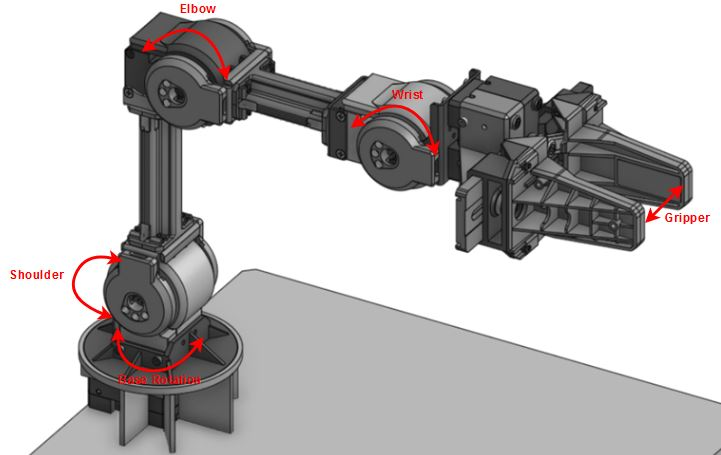
\includegraphics[width=6cm]{Arm Servo Joints.JPG}
        \caption{Location of robotic arm joints}
      \end{subfigure}%
      \begin{subfigure}{.5\textwidth}
        \centering
        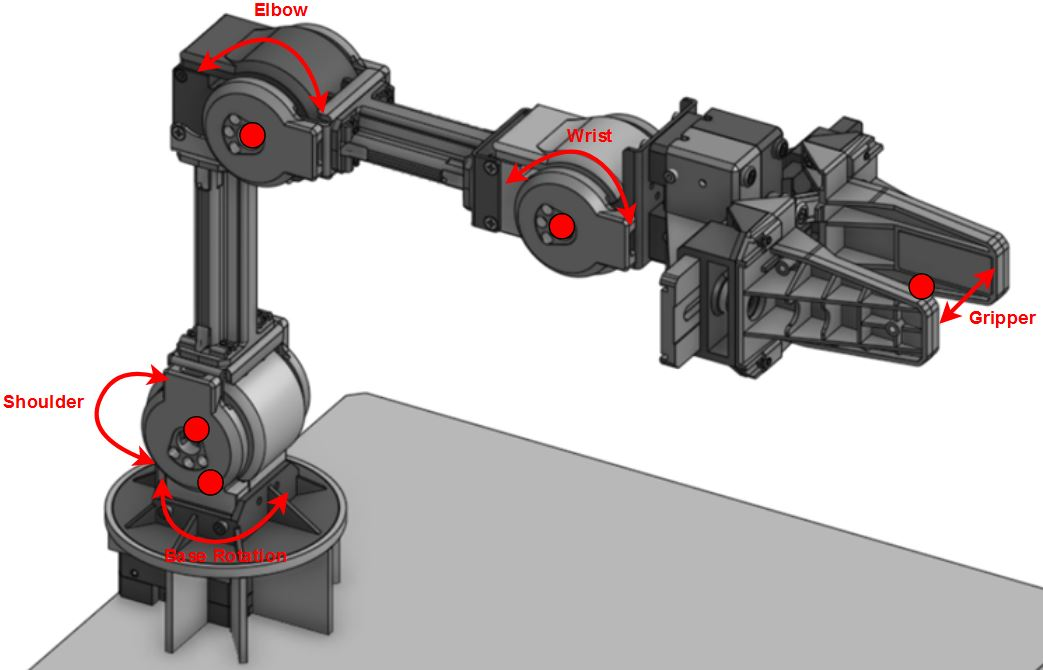
\includegraphics[width=6cm]{Arm Servo Joint with frames.JPG}
        \caption{Proposed locations of joint coordinate frames}
      \end{subfigure}
  \end{figure}
  
    
    \item Particular care has been placed on the position of the robotic arm's
    end effector. Particularly, the team discussion has been whether the end
    effector should be at the tip or the middle of the gripper.
    \begin{figure}[h]
        \centering
        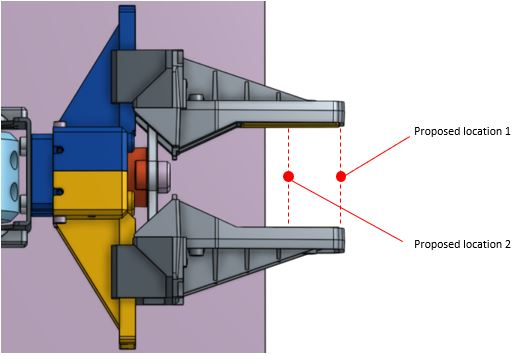
\includegraphics[width=5cm]{Effector location.JPG}
    \end{figure}
\end{itemize} 

Design decisions:
\begin{itemize}
    \item Base servo is vertically raised by $0.0613$m from the base frame to
    coincide with the rotating joint 

    \item End effector is chosen to be assigned to "Proposed location 2" as that
    gives the most secure grip with picking up items. \textbf{Care has to be taken to
    account for the extra $0.0152$m space from "Proposed location 2" to
    "Proposed location 1"}
\end{itemize}


\begin{figure}[h!]
    \centering
    \begin{subfigure}{.5\textwidth}
      \centering
      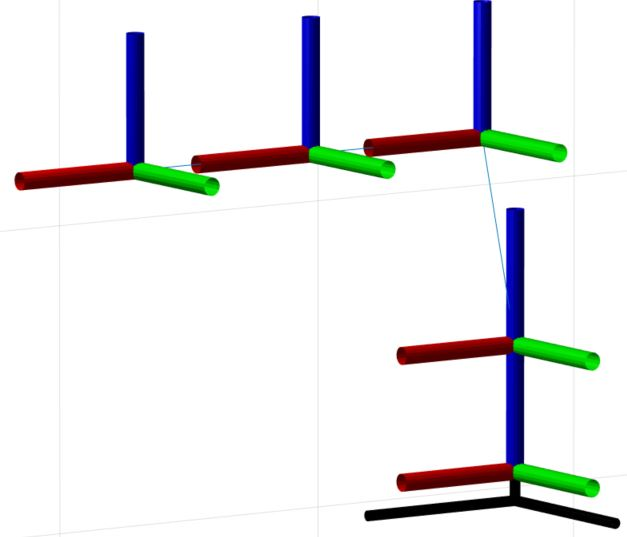
\includegraphics[width=5cm]{Line model.JPG}
      \caption{open-MANIPULATOR X Line model}
    \end{subfigure}%
    \begin{subfigure}{.5\textwidth}
      \centering
      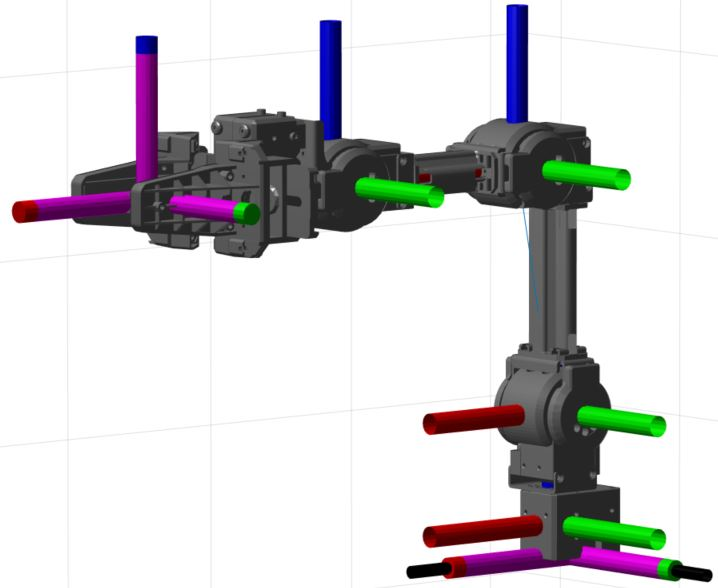
\includegraphics[width=5cm]{Robotic model.JPG}
      \caption{open-MANIPULATOR X 3D model}
    \end{subfigure}
\end{figure}

\vfill
\pagebreak

\subsection{Simulation: Graphical simulation of coordinate frames}

\subsection{Inverse Kinematics}

The Denavit-Hartenberg Parameter Table for the open-MANIPULATOR X robotic arm is
defined as:


\subsection{Simulation: Tracing a square on each cartesian plane}

    
\end{document}